\documentclass[11pt,a4paper, twocolumn]{article}
\usepackage[utf8]{inputenc}
\usepackage{graphicx}
\usepackage{subcaption}
\author{Eva Woodbridge and Angela Luo - ew----- wl17443}
\begin{document}
	\title{%
		Image Processing and Computer Vision \\
		\large The Dartboard Challenge}
	\maketitle 
	\begin{abstract}
		content...
	\end{abstract}
	\section{Viola Jones Object Detector}
	\subsection{Ground Truth and Visualisation}
		\begin{figure}[h!]
			\centering
			\begin{subfigure}[b]{0.4\linewidth}
				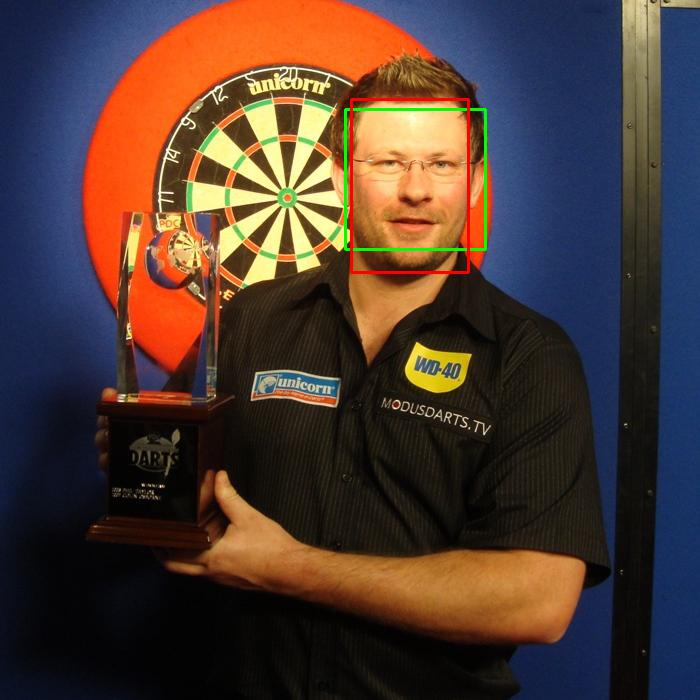
\includegraphics[width=\linewidth]{dart4_post.jpg}
				\caption{dart4.jpg}
			\end{subfigure}
			\begin{subfigure}[b]{0.4\linewidth}
				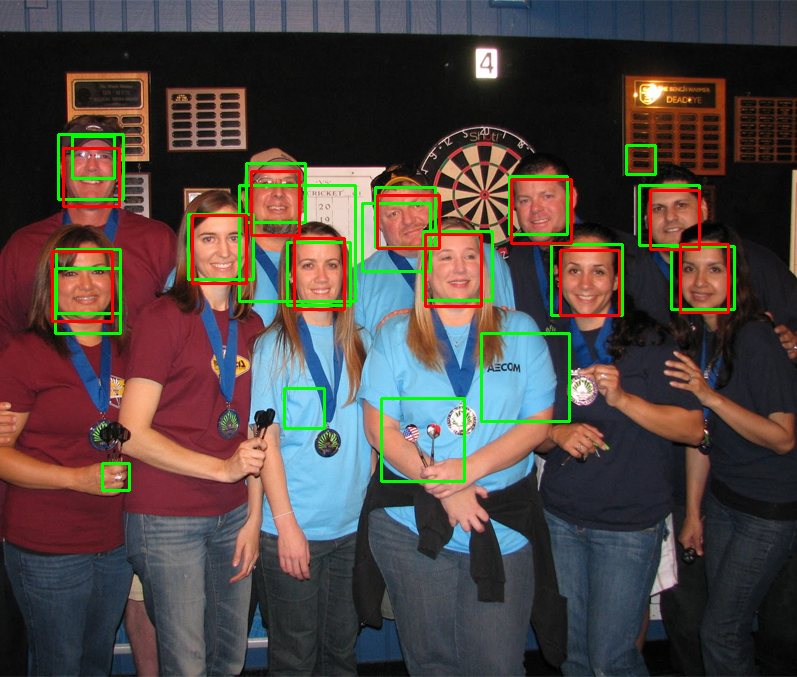
\includegraphics[width=\linewidth]{dart5_post.png}
				\caption{dart5.jpg}
			\end{subfigure}
			\begin{subfigure}[b]{0.4\linewidth}
				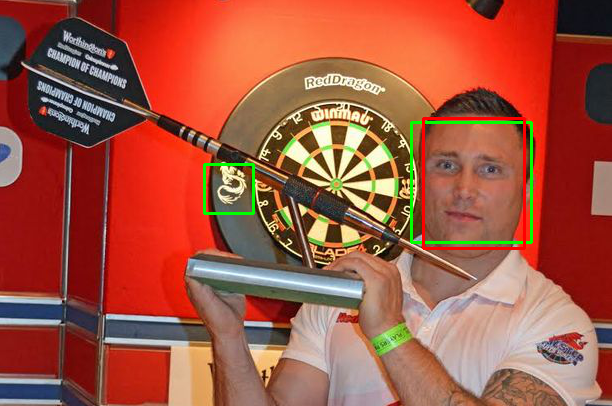
\includegraphics[width=\linewidth]{dart13_post.png}
				\caption{dart13.jpg}
			\end{subfigure}
			\begin{subfigure}[b]{0.4\linewidth}
				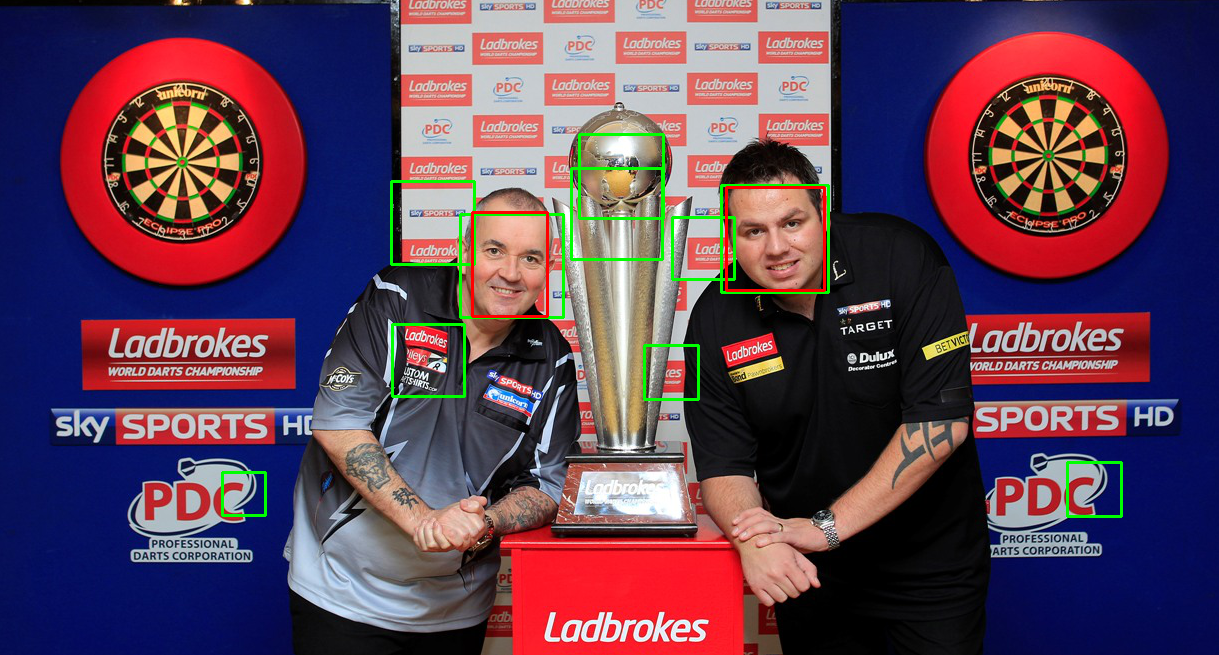
\includegraphics[width=\linewidth]{dart14_post.png}
				\caption{dart14.jpg}
			\end{subfigure}
			\begin{subfigure}[b]{0.4\linewidth}
				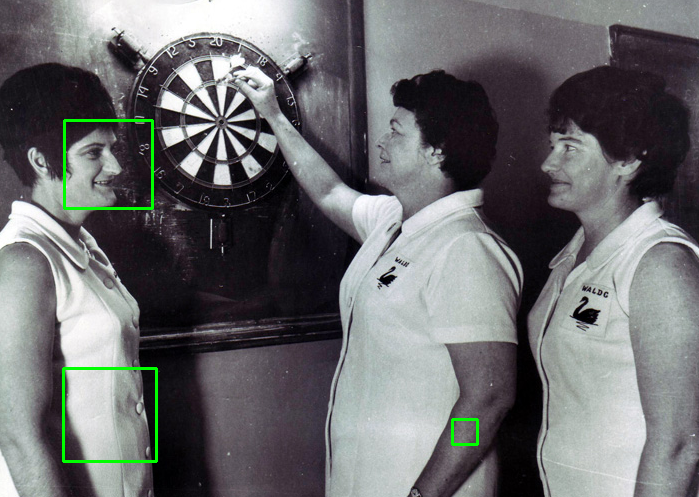
\includegraphics[width=\linewidth]{dart15_post.png}
				\caption{dart15.jpg}
			\end{subfigure}
			\caption{Five  result  images  with bounding boxes of the ground truth (in red) and actually detected instances (in green) drawn around frontal faces}
			\label{fig:violajonesfaces}
		\end{figure}
	\subsection{IOU, TPE, F1-Score}
	\section{Building and Testing a Detector}
	\subsection{Training Performance}
	\subsection{Testing Performance}
	\section{Integration with Shape Detectors}
	\subsection{Hough Details}
	\subsection{Evaluation}
	\subsection{Detection and Pipeline}
	\section{Improving Our Detector}
	\subsection{Idea}
	\subsection{Visualize}
	\subsection{Evaluate}
\end{document}